\cleartooddpage[\thispagestyle{empty}]
% Redefined Commands and Environments
\renewcommand{\thechapter}{\thechapter}
\renewcommand{\thesection}{\thechapter.\arabic{section}}
\renewcommand{\thesubsection}{\thechapter.\arabic{section}.\arabic{subsection}}
\renewcommand{\thesubsubsection}{\thechapter.\arabic{section}.\arabic{subsection}.\arabic{subsubsection}}
\renewcommand{\thefigure}{\thechapter.\arabic{figure}}
\renewcommand{\thetable}{\thechapter.\arabic{table}}
\renewcommand{\theequation}{\thechapter.\arabic{equation}}
\appendix

\chapter{Cross Section Upper Limits}

\input{images/ulimit/ulimittable.tex}

\chapter{VERITAS Data Run Numbers}\label{app:runlists}

\input{images/runlists/runlists.tex}

\chapter{Effect of Stars}\label{app:starpixels}

  Understanding the camera's background is important for accurately modeling extended sources like dark matter halos.
  The camera's background shape is due to the performance of many individual camera pixels working together.
  VERITAS onsite operators had, in the past, noted that for apparent visible magnitude $m_V :$ 6-8 stars, the camera pixels they illuminated would have a higher average current.
  This causes higher pedestal variations in the affected pixels, which decrease how often the pixel participated in shower images.
  In addition, if a star with $m_V < 6$ was in the field of view, it would cause a high enough current in the pixel to trigger a safety system that lowers its voltage to zero, to prevent it from being damaged.
  For particularly bright stars, such as $m_V \leq 3$, several pixels can be disabled at any given time.

  Compounding this effect is that, since the telescope camera is fixed to the ground, the sky rotates around the camera center.
  This means that over a single 30 minute observation the field of view rotates around the camera center, and each star in view disables successive camera pixels as it passes over them.
  The camera rechecks these disabled pixels roughly once per minute by turning their voltage back on and monitoring the current, and resetting it to zero if the current is still above the threshold.

  These effects imply that to study the effect of stars, one must study the effect of high-current and disabled camera pixels, and use this information to construct the effect of stars.
  In the following section, the effects of disabled camera pixels are studied.

\section{Effects of Disabled Pixels}

% see calculations/disabledpixel_obstime , those 250 crab runs turned into about 13.5 observation hours
To examine the effects of disabled pixels, \nicetilde13 hours of Crab Nebula observations were reconstructed twice.
The first analysis was with the default analysis chain settings, and the second time with a single pixel disabled in all four telescopes.
This mimics the effect of having a star in the field of view that is bright enough to disable a pixel.
The purpose of this study is to examine how many events are lost due to a dead pixel.
If there are bright stars near the Galactic Center, or a large number of disabled pixels in the data, the telescopes would be less sensitive to any dark matter halo.

After gamma-hadron cuts are applied to both sets of events, studies can be performed on events that only appeared in one set and not the other.
Some events may only pass gamma-hadron cuts with the pixel enabled ($P_e$), while others only pass when the pixel is disabled ($P_d$).
Events that are present both when the pixel is disabled and enabled can also be tested to see how far their reconstructed position moved in the camera.

In Figure~\ref{fig:dpix_rel_camera}, the relative event rate in the camera is plotted when pixel 115 is disabled in all four telescopes.
This relative event rate is calculated by binning all $P_d$ and $P_e$ events by their reconstructed position in camera coordinates.
Then, for each camera coordinate bin, the ratio of the number of events $\frac{P_d}{P_e}$ is calculated.
It can be seen that there is a loss of events near the disabled pixel (the black circle), with a rate closer to 100\% the farther one goes from the disabled pixel.

\begin{figure}[!ht]
  \centering
  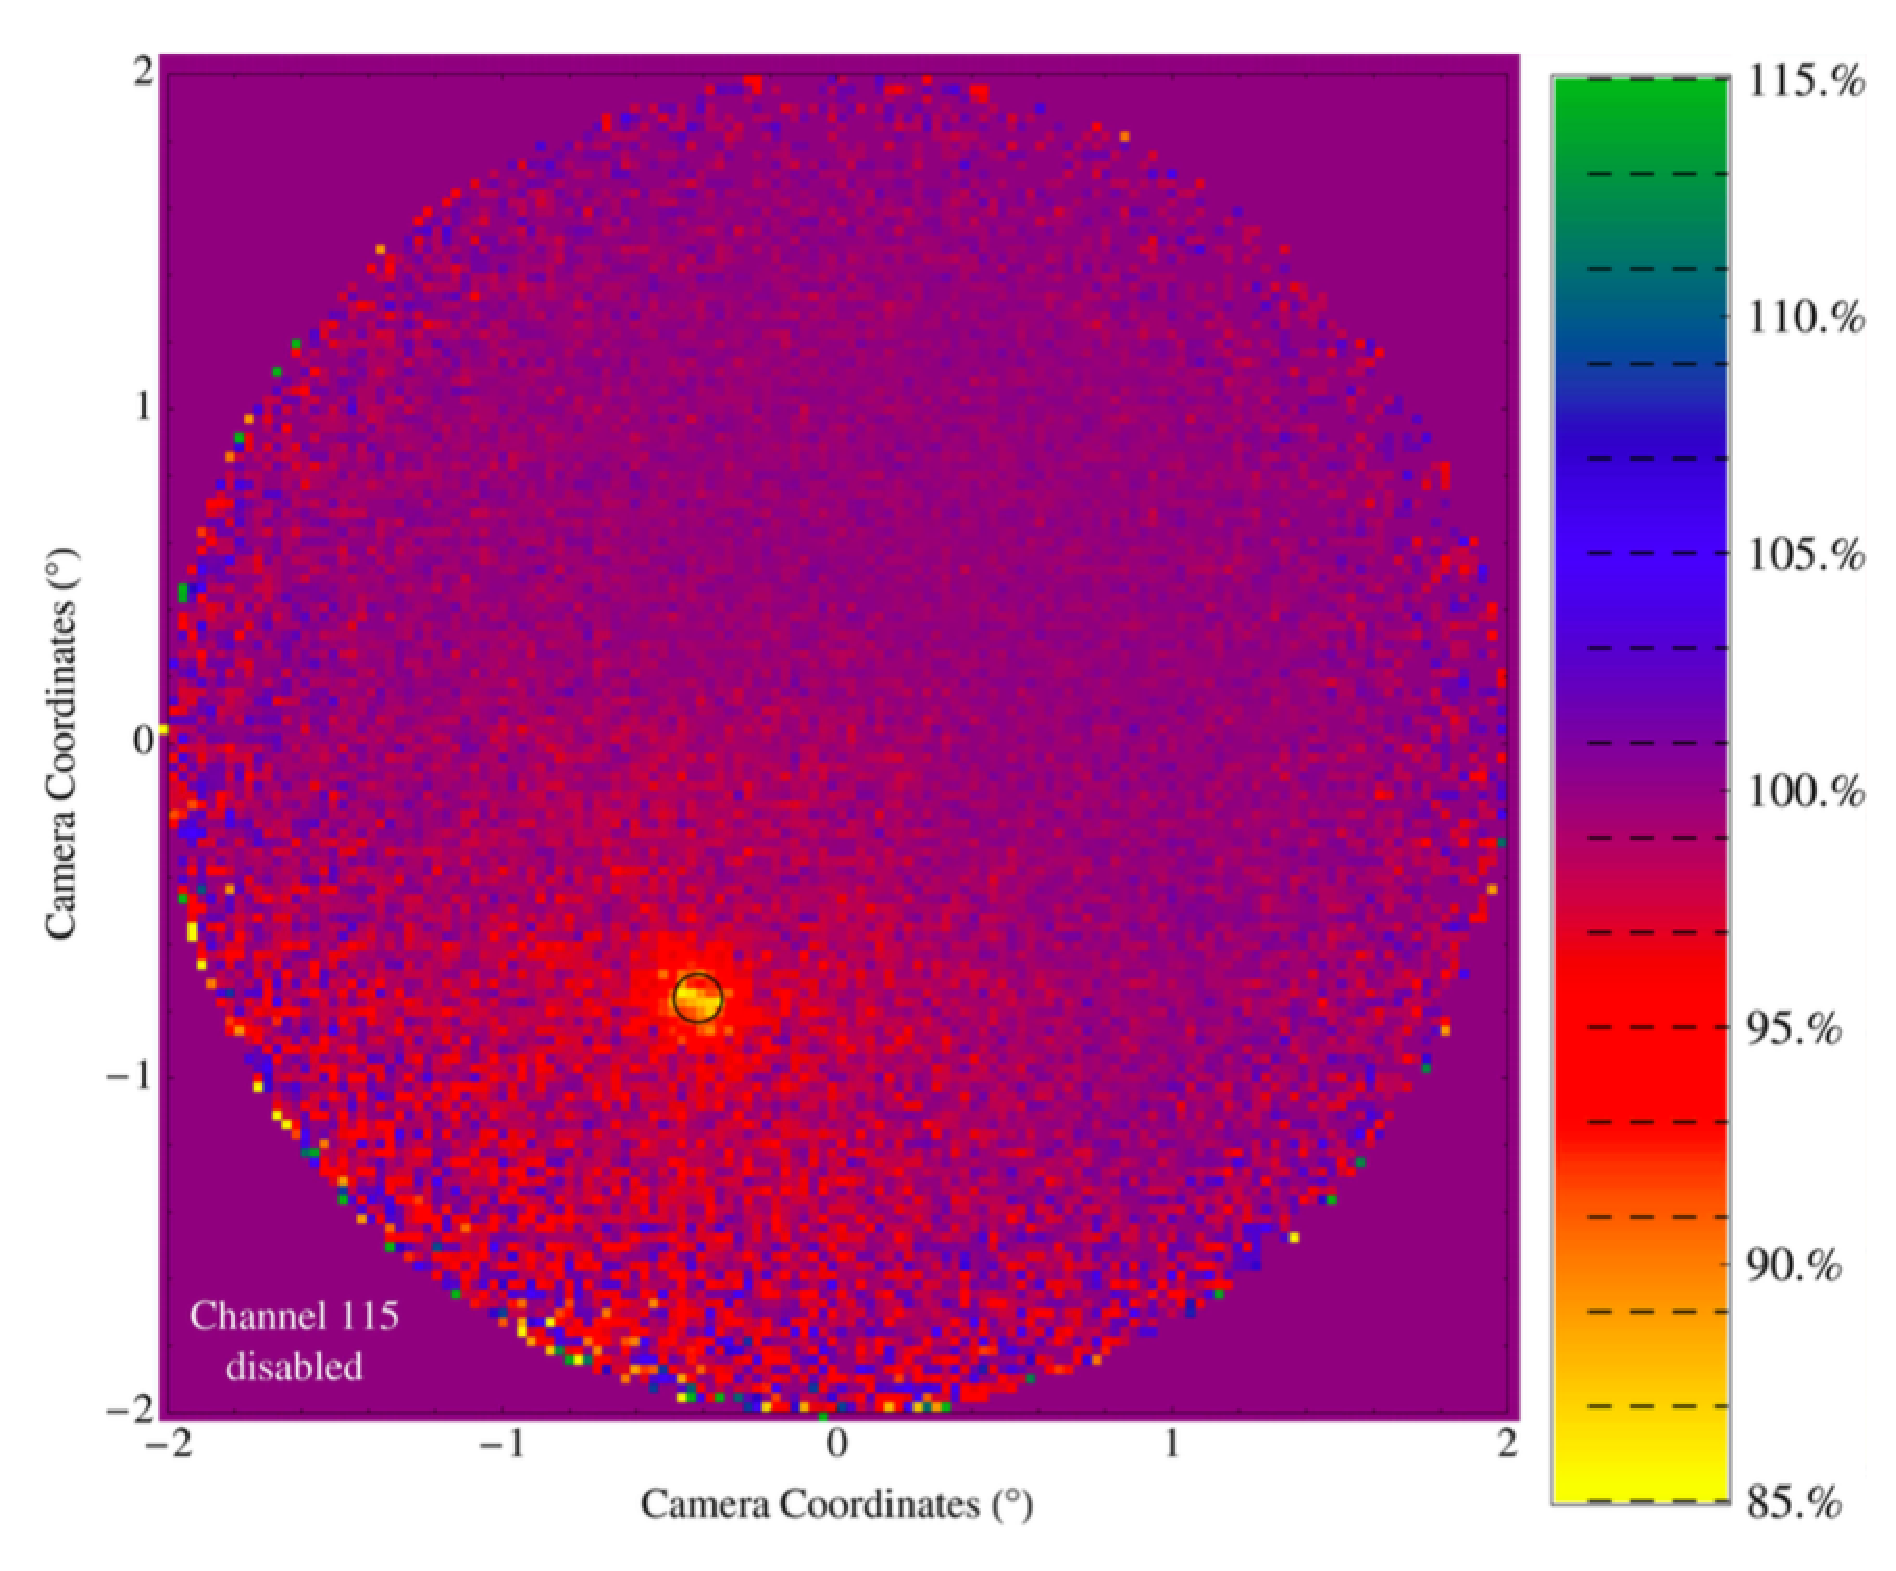
\includegraphics[width=0.8\textwidth]{images/disabled_pixel/relativerate_camera}
  \caption[Relative Event Rate After Disabling Camera Pixels]{
    Relative number of reconstructed events in the camera (squares) when pixel 115 disabled (denoted by the black circle) in all four telescopes, relative to having all pixels enabled.
    Camera coordinate axes are parallel to azimuth and elevation.
    It should be noted that squares in this plot are showing the reconstructed positions of events, which can be resolved to positions smaller than one PMT pixel.
  }
  \label{fig:dpix_rel_camera}
\end{figure}

When these bins are combined radially around the disabled pixel, a clear loss of events is visible in Figure~\ref{fig:dpix_rel_radial}.
From this, it can be seen that at \ang{0.1} from the disabled pixel, the relative event rate is almost 7\% lower than when the pixel was enabled.
From a area-weighted average of all bins within \ang{0.33} of a pixel, the average event rate is approximately 3.1\% lower than when the pixel is enabled.
Over the entire field of view, disabling one pixel in all four telescopes resulted in 0.7\% fewer events (14900 events vs 15010 per average \SI{20}{minute} observation).

\begin{figure}[!ht]
  \centering
  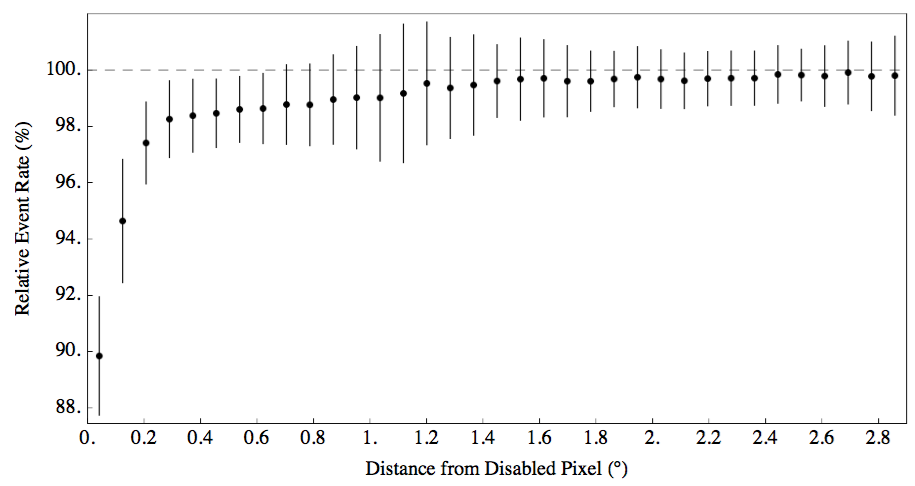
\includegraphics[width=0.8\textwidth]{images/disabled_pixel/relativerate_radial.pdf}
  \caption[Relative Event Rate After Disabling Camera Pixels]{
    Event rate in the camera with pixel 115 disabled (denoted by the black circle) in all four telescopes, relative to having all pixels enabled.
    The x-axis shows the angular distance from the disabled pixel.
  }
  \label{fig:dpix_rel_radial}
\end{figure}

% see images/disabled_pixel/dead_pixel_calcs/calc.py
% dead pixel signature: crab run 88721, pixel 216 (voltage gets dropped by more than 50%)
% also see DQM page for that run (AvgTraceMap plots)
% 1.3% of pixel-minutes are lost due to disabled pixels (18083/1427286 = 0.0126)
% calc this for each runlist as a measure of how few star-disabled pixels there are
% point out this is a better measure of star effects, since this is lower-level than stars,
%   its how many pixels are disabled for any reason

% in /Volumes/Charybdis/Research/Dead Pixel Statistics/Run Pixel Voltages/
% each run's data is downloaded via veripy.VeritasDB().run2pixelvoltagecurrents(run)
%
% numerator   : $ cat crab/*.dat | awk '$6>0 && $6<600 {print $6}' | wc -l
% denominator : $ cat crab/*.dat | awk '$6>0           {print $6}' | wc -l
% 
% $6>0   : when an entire telescope is cut or offline, all the voltages are -9999ish, so these are removed first
% $6<600 : 600V is roughly the threshold between enabled and disabled pixels.
%          Most enabled voltages are around 1000V.
%          Most disabled pixel voltages are around 300V.
%
% ratio of pixel-minutes where pixel voltage < 600V / total pixel-minutes
% Crab       runs:  37701pixmin/ 2245377pixmin = 1.679% pixel-time lost due to disabled pixels
% Sgr A*     runs: 127611pixmin/14553421pixmin = 0.877% 
% Sgr A* Off runs:  28813pixmin/ 2458631pixmin = 1.172%

While this single-pixel loss-of-events effect was notable, it was also quite small.
This was because for the Galactic Center analyzed in this thesis, there were relatively few disabled pixels.
For the three observing targets described in Chapter~\ref{chapter:analysis}, the amount of time pixels spent disabled was calculated.
The Crab Nebula observations had a total of 2,245,377 pixel-minutes, while 37,701 pixel-minutes were lost due to pixels being disabled, about 1.68\%.
This 1.68\% equates to a loss of 8.4 pixels (out of 499) in each telescope for the duration of an observation.
For the Sgr A* Off data, the loss rate was lower at 1.17\%, equivalent to losing 5.8 pixels in each telescope.
For Sgr A*, 0.88\% of pixel-minutes were lost, equivalent to losing 4.4 pixels in each telescope.

As these disabled pixels are mostly caused by bright stars, a search of bright stars near each observing source may shed some light on why the Crab Nebula loses 1.6\% of its pixels, while Sgr A* and Sgr A* Off lose less.
Table~\ref{tab:brightstars} shows the brightest stars near each observing source brighter than V${}_{mag}<6.5$.
While the Crab Nebula has several bright stars including HIP26451 with V${}_{mag} = 2.97$, Sgr A* Off and Sgr A* only have dimmer stars (V${}_{mag}$ 4.28 and 4.53, respectivly).
Since a one pixel disabled in all telescopes resulted in 0.7\% fewer events, and the Sgr A* observations in this analysis have \nicetilde{}4.4 pixels disabled, a rough estimate for the events lost due to stars near Sgr A* is approximately 3\%.
Crab Nebula observations, with 8.4 lost pixels, lose approximately 5.9\% of its events.
Note however, that the majority of these event losses are not gamma rays from the observing target, but are instead lost background events near (<\ang{0.5}) the position of the stars that disabled pixels.
A gamma-ray source that also emitted optical photons, or a gamma-ray source transiting across an optical one, or visa versa, would all be susceptible to having its flux underestimated due to this effect.
Due to the scarcity of bright ($V_{mag}<3$) visible stars and bright gamma-ray sources, this syzygy is extremely rare.
\begin{table}[t]
  \centering
  \begin{tabular}{|l|l|r|r|}
    \hline
    \textbf{Source} & \textbf{Star} & \textbf{Angle} & \textbf{V${}_{mag}$} \\ 
                    &               & [deg]             &                      \\
    \hline
    Crab Nebula & HIP26451 & 1.13 & 2.97 \\
                & HIP25539 & 1.60 & 4.88 \\
                & HIP26248 & 2.04 & 5.37 \\
                & HIP26072 & 1.55 & 6.19 \\
                & HIP26964 & 2.35 & 6.23 \\
                & HIP25806 & 0.99 & 6.29 \\
                & HIP26853 & 1.86 & 6.35 \\
                & HIP26616 & 1.17 & 6.42 \\
    \hline
    Sgr A* Off  & HIP85423 & 1.18 & 4.28 \\
                & HIP85084 & 0.87 & 5.30 \\
                & HIP85442 & 1.12 & 5.98 \\
                & HIP84445 & 2.08 & 6.20 \\
    \hline
    Sgr A*      & HIP87072 & 1.25 & 4.53 \\
                & HIP87836 & 2.60 & 5.76 \\
                & HIP87163 & 2.12 & 6.31 \\
                & HIP86725 & 1.24 & 6.40 \\
    \hline
  \end{tabular}
  \caption[Bright Stars in the Fields of View]{
    A list of nearby stars for each observing source in this analysis.
    The source column is star's closest source.
    The 2nd column is the star's Hipparcos catalogue code.
    The 3rd column is the angle between the star and the source, in degrees.
    The 4th column is the visual magnitude, taken from Ref.~\cite{hipparcos_catalogue}.
    Rows are sorted by source, then visual magnitude.
    Only stars brighter than V${}_{mag}=$ 6.5 are shown.
    % table generated with ~/Dropbox/Research/Thesis/images/disabled_pixel/stars_in_fov/fovstars.py
  }
  \label{tab:brightstars}
\end{table}

In Figure~\ref{fig:dpix_disappear}, the positions of events that were rejected by cuts are shown.
The white area indicates many events are lost in the area of the disabled pixel.
These events would have smaller images, and would be much more susceptable to being cut.

\begin{figure}[!ht]
  \centering
  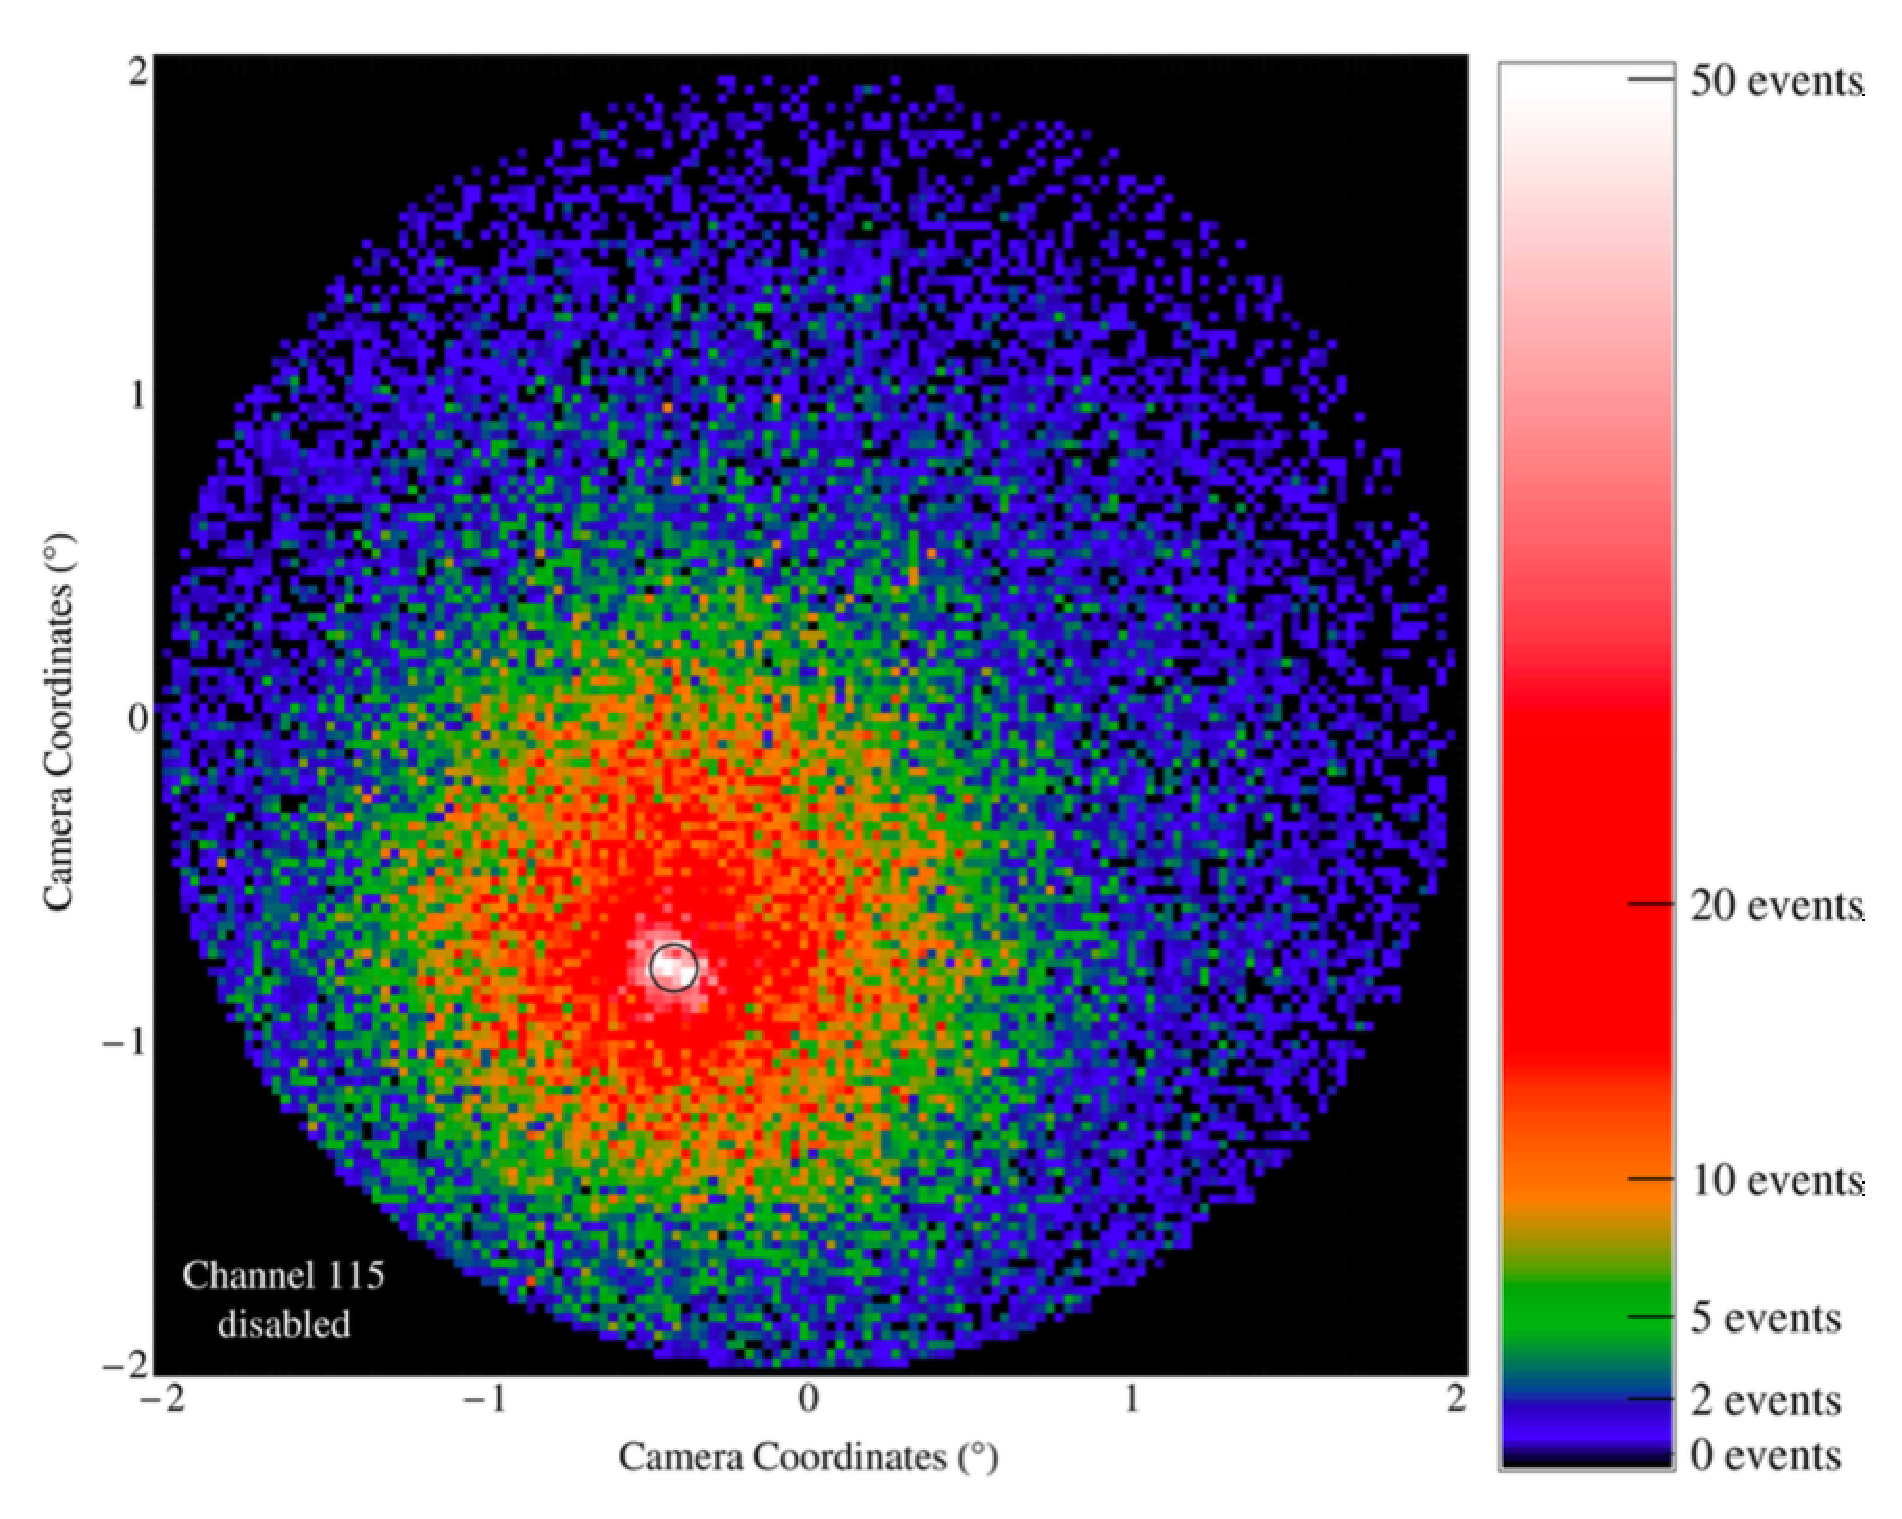
\includegraphics[width=0.8\textwidth]{images/disabled_pixel/disappearing_events}
  \caption[Events That Disappear when Disabling Camera Pixels]{
    Reconstructed positions of events that disappeared (squares) when pixel 115 (black circle) was disabled in all four telescopes.
    Positions are from their pixel-enabled reconstructed position.
  }
  \label{fig:dpix_disappear}
\end{figure}

In Figure~\ref{fig:dpix_appear}, the positions of events that are now able to pass cuts are shown.
It should be noted that these are not events that were 'created' by disabling a pixel.
Rather, they are events that, with the pixel enabled, did not pass cuts.
Now that the pixel is disabled, they do pass cuts.

What is also noticeable is that the highest concentration of lost events was in the pixel's area, whereas the highest rate for appearing events is actually in a ring with a radius of \nicetilde1.5 pixels around the disabled pixel.
This is probably due to the fact that disabling a pixel can make some images look thinner or wider, depending on where the disabled pixel is in the image.
A thinner image will look more gamma-like, making it more likely to pass cuts.
On the other hand, a wider image looks more hadron-like, and is less likely to pass cuts, causing some events to disappear.

\begin{figure}[!ht]
  \centering
  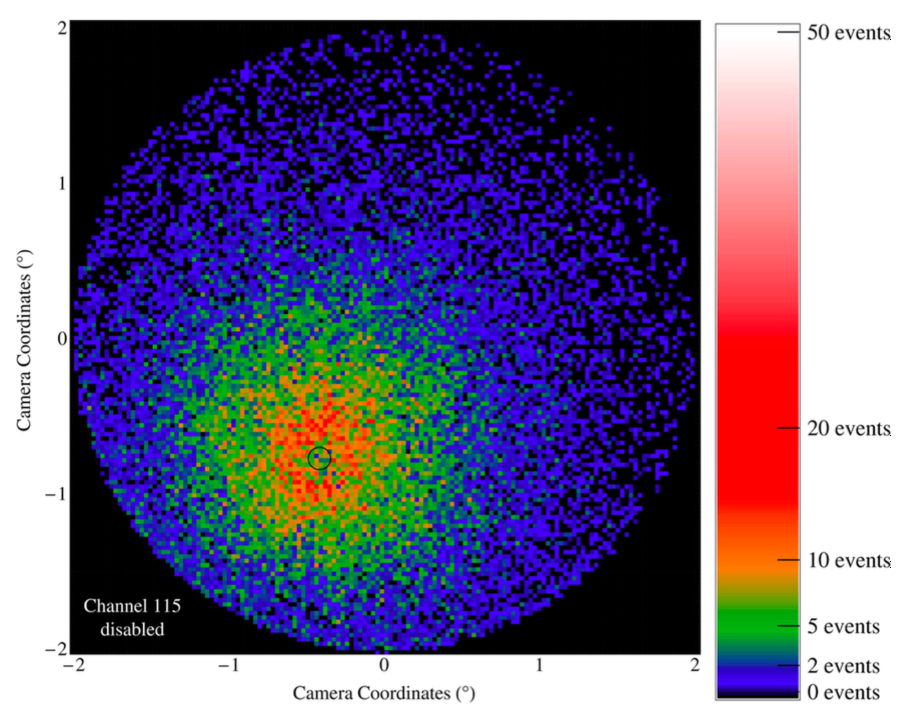
\includegraphics[width=0.8\textwidth]{images/disabled_pixel/appearing_events}
  \caption[New Events that Appear when Disabling Camera Pixels]{
    Reconstructed positions of new events (squares) that appeared when pixel 115 (black circle) was disabled in all four telescopes.
    Positions are from their pixel-disabled reconstructed position.
  }
  \label{fig:dpix_appear}
\end{figure}

In Figure~\ref{fig:dpix_move}, the movement of gamma-like events is shown, when pixel 115 was disabled in all four telescopes.
Only events which moved more than 10\% of the PSF are shown.
It should be noted that relatively few (0.7\%, or 117 out of the 15010 events in an average 20-minute long Crab Nebula run) move more than this, and the events that do move are mostly ones with non-compact image shapes that are amputated when a pixel is disabled.

What can be learned from this is that a negligbly small number of events' positions depend on a given pixel.
Though, unexpectedly, disabled pixels have an impact on events' reconstructed positions, even on the other side of the camera.
This may imply that the gamma-ray PSF is, to second order, dependent on the number and pattern of disabled pixels, though no studies were done to confirm this.

\begin{figure}[!ht]
  \centering
  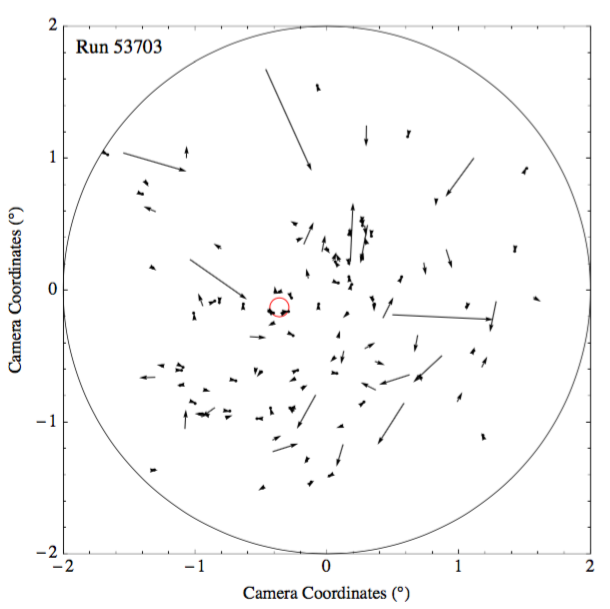
\includegraphics[width=0.7\textwidth]{images/disabled_pixel/moving_events}
  \caption[Event Movement After Disabling Camera Pixels]{
    Reconstructed events that moved when pixel 115 (denoted by the red circle) was disabled in all four telescopes.  
    Arrows point from the pixel-enabled position to the pixel-disabled position.
  }
  \label{fig:dpix_move}
\end{figure}

As the acceptance for a particular event and the event's effective area are strongly related, the loss of acceptance also means a loss of effective area near the pixel.
This can have effects on the energy reconstruction.
Additionally, for CTA and its projected \ang{7} diameter field of view, more stars will be in the field of view, implying there will be more camera pixels affected by their light.

\textbf{An important concept to learn from these studies is that the PMTs in the camera work together as a whole to reconstruct events, and the loss of one PMT can affect the reconstruction of events anywhere else in the camera.}
From these studies, it can be seen that the loss of a single pixel does not significantly reduce the overall event rate, but does decrease the event rate by \nicetilde{}3\% near (<\ang{0.3}) the position of stars that are brighter than magntiude 6.5.
For the Galactic Center, only 1\% of the pixels are disabled, equivalent to 5 pixels in each telescope on average.
% 2320620 disabled pixelseconds out of 214657920 total pixelseconds in the Sgr A* runlist
% 2320620 / 214657920 = 0.0108 fraction of time lost
% 499 * 0.0108 = 5.38 pixels in each telescope
% see $VERIPY/thesis/analysis/find_dead_pixels_near_GC/find.py
As this study indicates the number of events lost is small, and there are relatively few dead pixels in the Galactic Center's field of view, the effect of dead pixels was ignored in the dark matter search.

Another reason these disabled pixels are not accounted for is discussed in Chapter~\ref{chapter:analysis}, where small disabled-pixel effect is dwarfed by the problems with modeling how the background rate is affected by the atmospheric gradient.
Future analyses may be able to account for these effects in their models of the background rates and effective areas.

Future studies could also compare how events move in energy when a pixel is disabled.
Another study might investigate how the reconstructed shower-telescope distance changes, since a shower with fewer pixels will look further away, and may be reconstructed differently.
Another possibility is that, for VERITAS or future CTA observations where pixels are disabled (either due to stars or maintainance), customized background models can be constructed that account for the specific configuration of disabled pixels.
Since the disabled pixel information (which pixels and the disable/enable times) is saved as part of regular observation monitoring, this can be used to apply gaussian event-rate penalties to any background models.
In general, when a pixel is disabled, it is expected that lower energy events and showers further away will be more vulnerable, and will show stronger differences than higher energy events or closer showers.




